%-----------------------------------------------%
% Início do plano de aula
%-----------------------------------------------%
\thispagestyle{empty}
\begin{center}
	\begin{minipage}[!]{\linewidth}
        \begin{minipage}[!]{.19\linewidth}
            
\includegraphics[width=\linewidth]{img/logo.png}           
        \end{minipage}
        \begin{minipage}[!]{.8\linewidth}
            \center
            \ABNTEXchapterfont\normalsize\MakeUppercase{\imprimirinstituicao}
            \par
            \vspace*{10pt}                     
            \ABNTEXchapterfont\normalsize\MakeUppercase{\centro}
            \par
            \vspace*{10pt}           
            \ABNTEXchapterfont\normalsize\MakeUppercase{\disciplina}
        \end{minipage}        
    \end{minipage}
    \\ \vspace{0.5cm}
    \rule{\textwidth}{.5pt}   
\end{center}
    \textual
    \begin{center}
      \section{Teoria Ondulatória da Luz}
      \par
    \end{center}
    
    \noindent \textbf{Estagiário(a): }\imprimirautor 
    
    \noindent \textbf{U.E.: }EEB Giovani Pasqualini Faraco
    
    \noindent \textbf{Série: }2º Ano\hfill{}\textbf{Turma: }2º--5
    
    \noindent \textbf{Aula:} 006\hfill{}\textbf{Data:} 04/11/2022\hfill{}\textbf{Duração:} $45\min$
    \rule{\textwidth}{.5pt}
    \bigskip{}  
    

    \noindent
    \begin{center}
      \textbf{Lei de Snell-Descartes}
    \par\end{center}
    \vspace{20pt}
    \noindent \textbf{Resumo da aula:} Nesta aula apresentaremos o modelo alternativo para os fenômenos luminosos, no que tange a sua velocidade de propagação, tendo por base o modelo ondulatório e o princípio de Huygens. A Lei de Snell-Descartes será demonstrada matematicamente, bem como sua previsão para a velocidade da luz. Por fim faremos o confronto entre as previsões deste modelo e o modelo corpuscular obtido na aula 03.
    \smallskip
    \par\noindent \textbf{Habilidades BNCC:} EM13CNT201.
    \medskip
    \subsection*{Objetivo de Aprendizagem}
    \begin{itemize}
        \item Conhecer o modelo ondulatório da luz;
        \item Diferenciar o modelo ondulatório do modelo corpuscular da luz;
        \item Compreender a formulação da Lei de Snell-Descartes e a importância do Princípio de Huygens para esta formulação.
    \end{itemize}    
    \bigskip{}    
    \noindent \textbf{Núcleo Conceitual:} \emph{Teoria ondulatória da luz; reflexão e refração.}
    \newpage
    

    \section*{Procedimento Didático} 
    \noindent\emph{1º Momento:} Problematização Inicial
    \par\noindent\rule{.3\textwidth}{.5pt}  
    \par\noindent\textbf{Tempo previsto:} 10 minutos
    \smallskip
    \par\noindent\textbf{Dinâmica:} Recordar as simulações feitas na primeira aula, atentar-se ao ponto em que virão o raio de luz se aproximando na normal, nos caso da luz propagando-se de um meio mais denso que o ar e o contrário quando inverteu-se os meios, a figura \autoref{fig:phet-a} ilustra os casos para o vidro.
    
    \vspace*{10pt}
    \begin{figure}[!ht]        
        \centering              
        \subfloat[\label{fig:phet-1}]{
            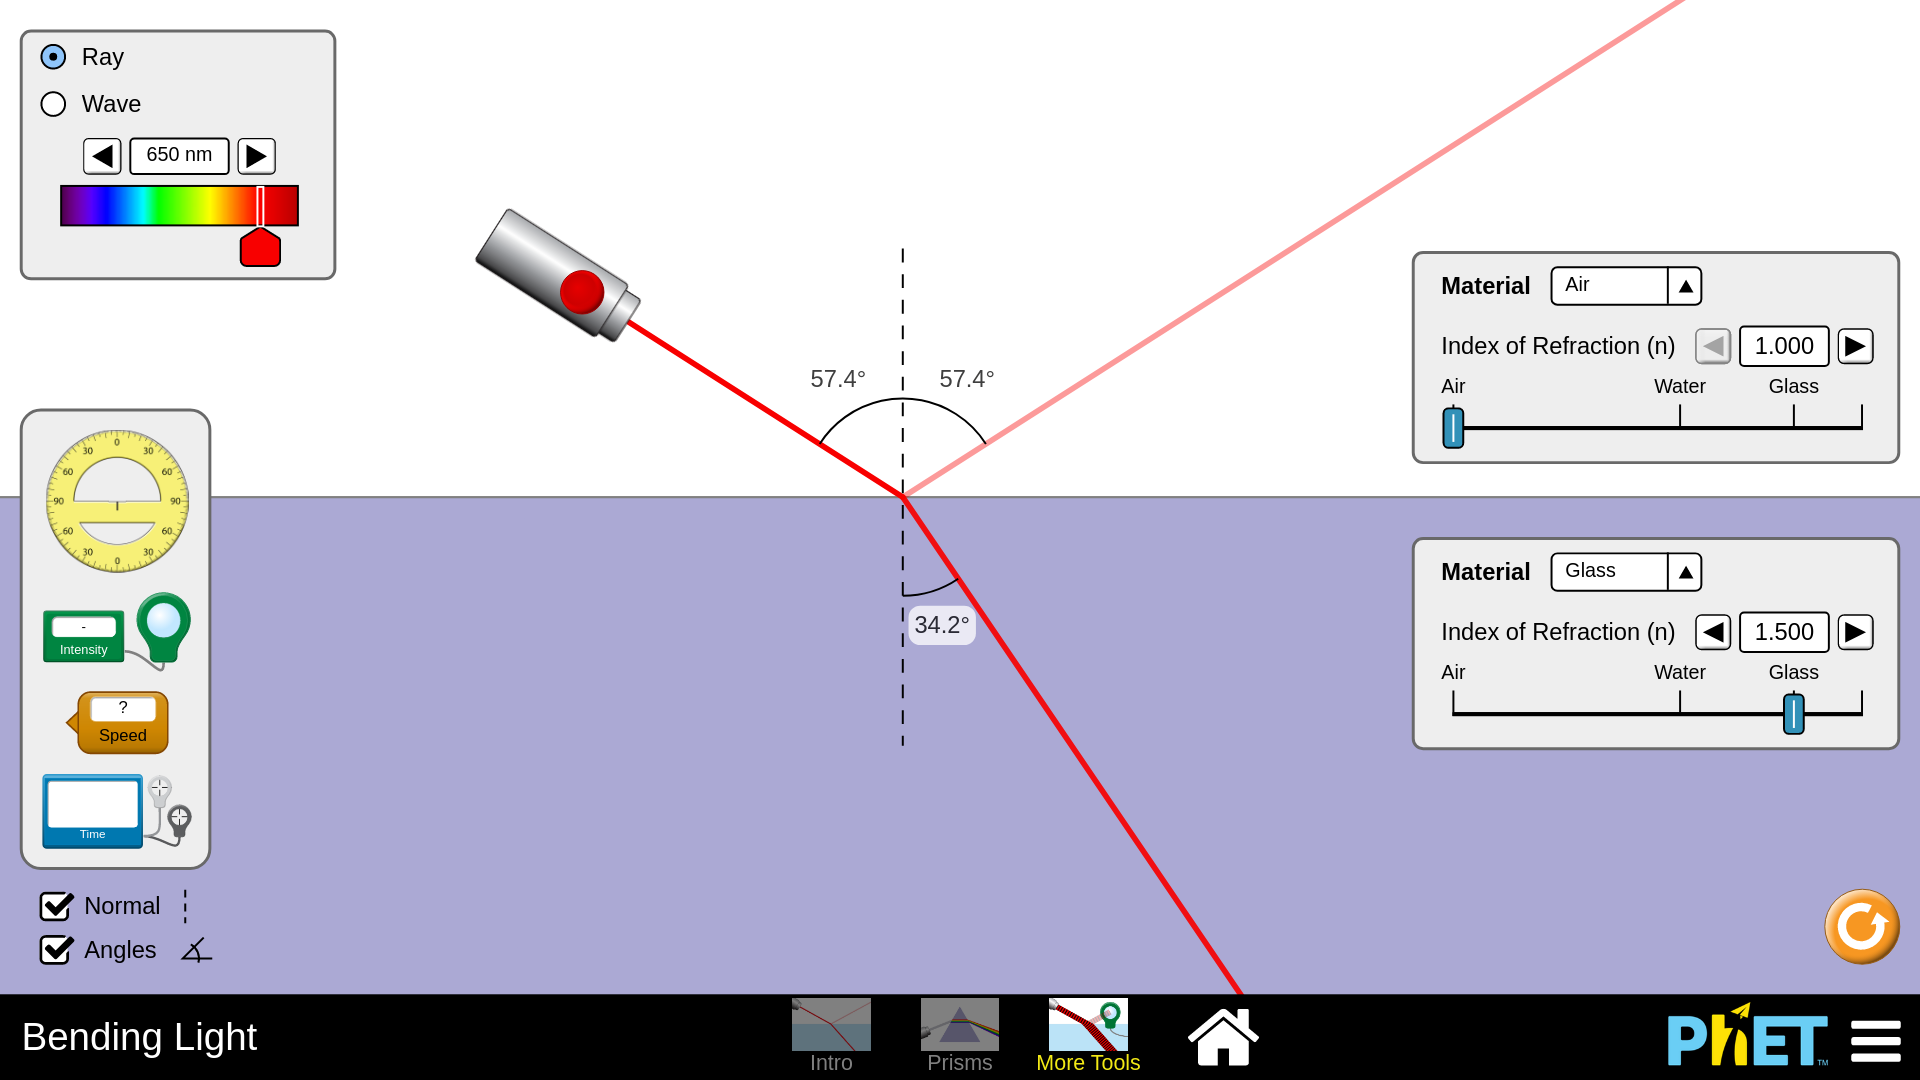
\includegraphics[width=.45\textwidth]{img/phet-1.png}
        }\hfill
        \subfloat[\label{fig:phet-2}]{
            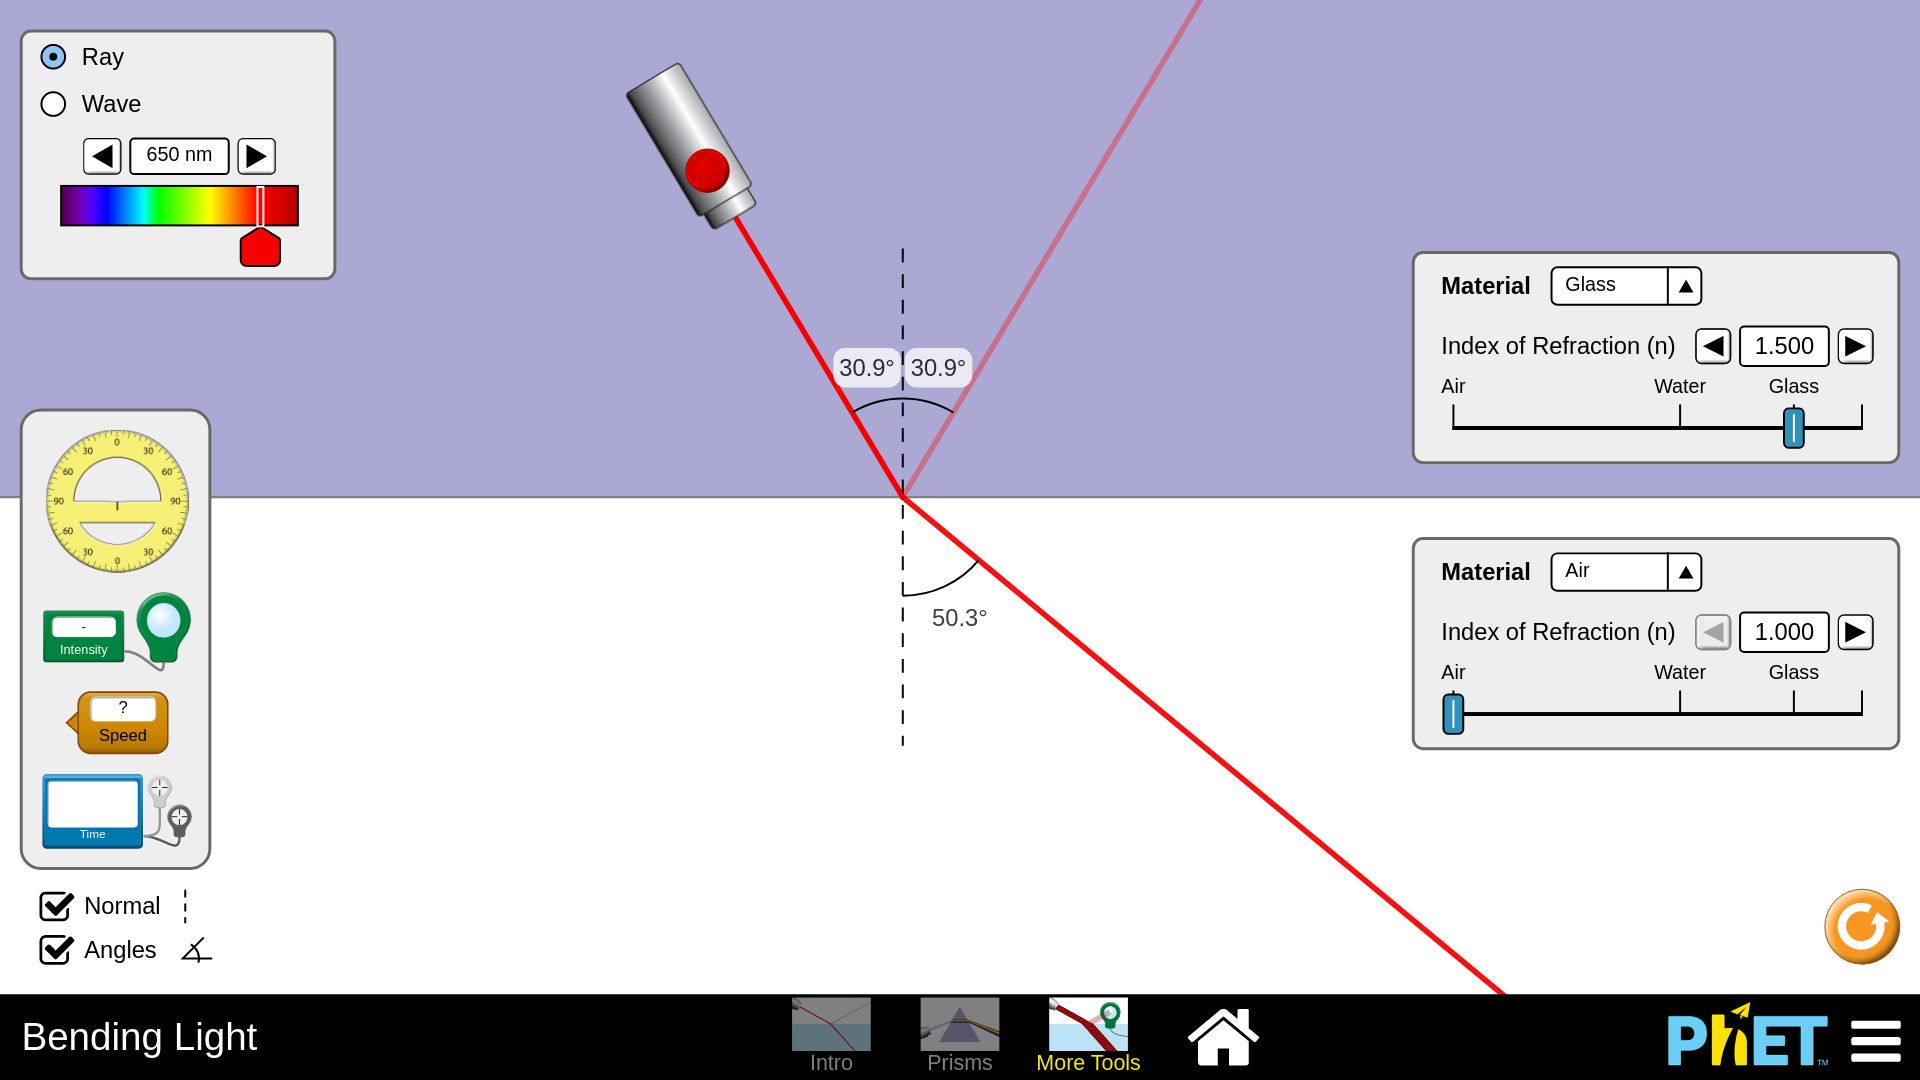
\includegraphics[width=.45\textwidth]{img/phet-2.png}
        }        
        \caption{Simulação \emph{Phet} em (a), feixe luminoso partindo do ar para o vidro, raio refratado aproxima-se da normal ao ponto de contato e em (b), feixe luminoso partindo do vidro para o ar, raio refratado afasta-se da normal ao ponto de contato.}
        \label{fig:phet-a}
    \end{figure}
    \vspace*{10pt}

    Recorda-los que foi associada esta mudança de trajetória que a luz faz, com a mudança na sua velocidade de propagação em cada meio.

    Recorda-los ainda, da previsão newtoniana para a velocidade da luz, nos casos em que a mudança de meios ocorre do ar para água, expressa pela relação

    \begin{align}
        v_{0}<v_{f}
    \end{align}
    em que $v_0$ é a velocidade da luz no ar e $v_f$ é a velocidade da luz na água (ou em qualquer outro meio mais denso).
% Segundo os autores é nessa etapa que se apresentam questões
% e/ou situações para discussão com os alunos, visando relacionar o estudo de um conteúdo com
% situações reais que eles conhecem e presenciam, mas que não conseguem interpretar completa ou
% corretamente porque provavelmente não dispõem de conhecimentos científicos suficientes. Ou seja,
% é na problematização que se deseja aguçar explicações contraditórias e localizar as possíveis
% limitações do conhecimento que vem sendo expressado, quando este é cotejado com o conhecimento
% científico que já foi selecionado para ser abordado (Delizoicov, Angotti e Pernambuco, 2002, p. 201).
% Portanto, esse primeiro momento é caracterizado pela compreensão e apreensão da posição dos alunos
% frente ao tema. É desejável ainda, que a postura do professor se volte mais para questionar e lançar
% dúvidas sobre o assunto que para responder e fornecer explicações.
    \newpage
    \bigskip{}
    \noindent\emph{2º Momento:} Organização do Conhecimento
    \par\noindent\rule{.3\textwidth}{.5pt}  
    \par\noindent\textbf{Tempo previsto:} 20 minutos
    \smallskip
    \par\noindent\textbf{Dinâmica:} Construir a dedução de forma dialogada usando o esquema representativo da \autoref{fig:snell-deducao}
    
    \vspace{10pt}
    \begin{figure}[!ht]        
        \centering              
        \subfloat[\label{fig:snell-deducao-a}]{
            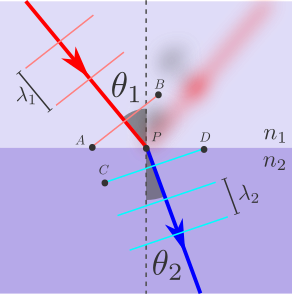
\includegraphics[width=.4\textwidth]{img/snell-1.png}
        }\hspace{20pt}
        \subfloat[\label{fig:snell-deducao-b}]{
            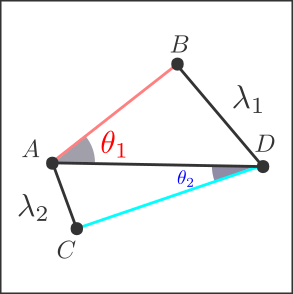
\includegraphics[width=.4\textwidth]{img/snell-2.png}
        }        
        \caption{Esquema representativo da lei de Snell, em (a) as frentes de onda incidente estão representadas por retas paralelas a direção de propagação da onda representada em vermelho, já as frentes de onda em azul representam a parte da onda refrata no material. Em (b) os triângulos $\triangle ABD$ e $\triangle ACD$ formados pelas frentes de onda incidente, refratada e a superfície do meio, são semelhantes.}
        \label{fig:snell-deducao}
  \end{figure}        
  \vspace*{10pt}

  Com o auxílio das figuras acima, extrair a relação
  \begin{align}
  \label{eq:snell-comprimento-de-onda}
      \frac{\sin\theta_1}{\sin\theta_2}&=\frac{\lambda_1}{\lambda_2}
  \end{align}
  Interpretar a eq. \eqref{eq:snell-comprimento-de-onda} em conjunto com os alunos e questioná-los o que se espera que ocorra com os comprimentos de onda $\lambda_1$ e $\lambda_2$ quando $\theta_1<\theta_2$ \emph{(fenômeno de dispersão)}.

  Relacionar a dispersão com os fenômenos da formação do arco-íris e da decomposição da luz branca no prisma de Newton.

    

% Delizoicov e Angotti (1990, p. 29) explicam que nesse
% segundo momento os conhecimentos de Física necessários para a compreensão do tema e da
% problematização inicial devem ser sistematicamente estudados sob orientação do professor.
% Definições, conceitos, relações, leis, apresentadas no texto introdutório, serão agora aprofundados.
% De acordo com Albuquerque, Santos e Ferreira (2015, p. 467) esse é o momento em que os
% conhecimentos científicos passam a ser incorporados nas discussões. Os alunos começam a
% desenvolver uma compreensão a respeito da problematização ou situação inicial. Entretanto, para que
% isso ocorra, materiais devem ser consultados e atividades devem ser sugeridas para complementar as
% discussões, no sentido de incentivar e melhorar a sistematização dos conhecimentos.
% Nessa perspectiva, Delizoicov e Angotti (1990) vêm ressaltar a importância de diversificadas
% atividades, com as quais se poderá trabalhar para organizar a aprendizagem. Sugerem exposições,
% pelo professor, de definições e propriedades, além de formulações de questões (exercícios de fixação
% como dos livros didáticos), textos e experiências. Neste sentido, atualmente poderíamos acrescentar
% as mídias tecnológicas, como televisão, vídeos, filmes, programas tecnológicos, aplicativos de
% celulares, simulações, entre outros, de modo a auxiliar no processo da sistematização do
% conhecimento.
    \newpage
    \bigskip
    \noindent\emph{3º Momento:} Aplicação do Conhecimento
    \par\noindent\rule{.3\textwidth}{.5pt}  
    \par\noindent\textbf{Tempo previsto:} 15 minutos
    \smallskip
    \par\noindent\textbf{Dinâmica:} Iniciar esta parte da aula relembrando a relação que foi encontrada para a velocidade de uma onda qualquer na aula 004
    \begin{align}
        v&=\lambda f
    \end{align}
    a partir da equação acima, obter $\lambda=v/f$ e substituir na \eqref{eq:snell-comprimento-de-onda} ficando com
    \begin{align}
    \label{eq:lei-de-snell-velocidades}
        \frac{\sin\theta_1}{\sin\theta_2}&=\frac{v_1}{v_2}
    \end{align}
    Questionar a relação entre $v_1$ e $v_2$ se $\theta_1>\theta_2$

    Finalizar a aula pedindo para que comparem este resultado com o que obtivemos na teoria corpuscular e ajustar a \eqref{eq:lei-de-snell-velocidades} para a sua forma usual dada por
    \begin{align}
        n_1\sin\theta_1&=n_2\sin\theta_2
    \end{align}
    em que os índices de refração absolutos de cada meio é $n_1=c/v_1$ e $n_2=c/v_2$.
    

% Essa última etapa aborda sistematicamente o
% conhecimento que vem sendo incorporado pelo aluno para analisar e interpretar tanto a situações
% iniciais que determinaram o seu estudo, como outras situações que não estejam diretamente ligadas
% ao motivo inicial, mas que são explicadas pelo mesmo conhecimento. (Delizoicov e Angotti, 1990,
% p. 31).
% Este é o momento importante para que os alunos encontrem relações entre os temas
% abordados, não apenas através dos conceitos, mas também de fenômenos que possam ter alguma
% conexão com as informações apresentadas. No entanto, o professor mantém a postura
% problematizadora, podendo trazer questionamentos que não foram levantados pelos alunos, como
% informações e problemas que surgiram do decorrer dos momentos. Além disso, este é um bom
% momento para o professor formalizar alguns conceitos que não foram aprofundados pelos alunos.
% (Albuquerque, Santos e Ferreira, 2015).

%-----------------------------------------------%
% FIM do plano de aula
%-----------------------------------------------%